\section{Key Management in Space DTNs}
\label{sec:survey}

Cryptographic key management is considered one of the most challenging problems in DTNs \cite{menesidou2016automated,menesidou2017cryptographic,ivancic2009security,asokan2007towards}. This section focuses on the study of the problem, defines a set of requirements to evaluate the solutions, and presents a survey of proposed key management systems for space DTNs.


It is already complex to deploy key management systems in traditional networks. The problem lies in the deployment and management of the infrastructure to support authenticated keys and not cryptographic algorithms \cite{al2003certificateless}. For DTNs, the problem is even worst.

A Key management system has fundamental goals: secrecy of keys and assurance of purpose \cite{martineveryday}.  DTNs present fundamental differences with traditional networks that make goals of protocols sometimes unclear or not simple to define, key management is not the exception.

Considering routing in DTNs to illustrate the problem. The problem of defining the goals of routing in DTNs is analysed in many papers \cite{ivancic2009security,fall2003delay,araniti2015contact}. In traditional networks, the purpose of routing is to select the best path between a source a destination. Routing protocols utilise the network state to calculate the best path according to one or more metrics. In space DTNs, the lack of connectivity and long propagation delays make the goals of routing more complex. The topology could change faster than the time that requires disseminate the topology updates. Routing still consists of selecting the next best hop until the destination, but the concept of best path is constrained. In this case, maximise the probability of bundle delivery could be the goal. \cite{araniti2015contact}. 


Several key management schemes were evaluated for this report. Many of these schemes adopted different metrics and requirements. Thus, it seems that the problem is not well understood and the it is not requirements are not clear. The rest of the section present a detail study of the key management problem in DTNs.

\subsection{Analysis of current Key Management Solution}


The first question that arises is whether symmetric or asymmetric keys should be used to support a key management system.  The section  \ref{sec:space} concludes that symmetric keys are the most suitable solution for current space missions. 

For the Interplanetary Internet is expected a scenario similar to the terrestrial Internet \cite{rationale2010requirements}. Multi-hop communications and cross-organisational domains are enhancements of the current interplanetary communications. Also, policies, rights, hierarchy, and administrative groups form part of the overall solution. The network might scale to thousands of nodes, and different space agencies will participate in the network. Considering this scenario, it seems more suitable a key management solution similar to the Internet rather than one based on symmetric keys. Furthermore, symmetric keys might not be even acceptable in a cross-organisational domain \cite{ivancic2009security}.

The research effort so far is based on asymmetric keys and DTN working groups stated the need for automated systems for distribution of authenticated public keys and revocations mechanism \cite{templin-dtnskmps-00}. Although there are ciphersuites based on symmetric keys in the security specification BSP \cite{ietf-dtn-bpsec-07}, there is a common consensus that asymmetric keys will be the preferred method for the Interplanetary Internet. 

In public key cryptosystems, a node must have a copy of the destination public key to encrypt the message, and the destination nodes must have the source node public key to verify integrity. Key distribution is not a sensitive operation in the sense that information is not secret.  Common techniques  to obtain public keys are \textbf{pushing} directly from the key owner and \textbf{pulling} from a usually trusted directory \cite{martineveryday}.

Relatively low delays on the Internet allow pushing and pulling to be effective to obtain public keys. For instance, TLS uses the pushing approach to retrieve the destination public key. After obtaining the public key, a node needs to check the validity of certificates with a Certificate Authority CA. Popular options for this validation process are certificate revocation list CRL or the Online Certificate Status Protocol OCSP, but these options require interaction with the CA which might not be available in deep space communications. 

Here should be noted as well that TLS, one of the most popular cryptographic protocol on the Internet, uses a handshake between the parties to retrieve public keys and negotiate some parameters for the session. Negotiation based protocols are discouraged for DTNs \cite{fall2003delay,cerf2007delay}.

There are modifications of OCSP to improve the message overhead, but these are designed to alleviate the overhead on certificates receivers, but the overhead is transferred to the other side of the communication. In Secure/Multi-purpose Internet Mail Extensions (S/MIME) sender could encapsulate its certificate as meta-data, but the receiver is expected to validate the information. S/MIME remove the communication between nodes but still require on-demands interactions with a trusted authority. 

There are other alternatives to public key management based on certificates. Templin \cite{templin-dtnskmps-00} states that web of trust might be an option for some types of DTNs, but more research should be done. For space-based networks, a model without a trusted authority is not acceptable \cite{viswanathan-dtn-pkdn-00,burleigh-dtnwg-dtka-01,ivancic2009security}.  

Another alternative widely explored for public key management in DTNs is Identity Based Cryptography IBC. This approach uses a direct derivation of the public key from the node ID and eliminates the requirement of public certificates.  Even though IBC eliminates some problems inherent to the management of public certificates, it introduces other issues such as key escrow and key revocation. These problems can be addressed but no without adding considerably overhead which questioned the benefits of IBC for DTNs.


Farrell \textit{et al.} stated that IBC does not solve the problem of key management \cite{irtf-dtnrg-sec-overview-06}; however, Asokan \cite{asokan2007towards} argue that IBC indeed solves the problem and provides an improvement in confidentiality services but not for authentication. In any case, proposal based on IBC are considered in this work.   


\subsection{Taxonomy of key Management in DTN}

A key management solution for DTN in space has the same requirement as any key management system along with extra considerations for the hostile environment. This section focuses on understanding why the problem is different from terrestrial networks as the Internet, define the requirements, and classify the solutions. 



Key management includes a wide range of processes which together provide security to cryptographic keys.  The problem of secure administration of cryptographic keys is complex but well-understood on terrestrial networks. Future space-based networks present two challenges to key management systems. Firstly, the network topology is dynamic; it consists of heterogeneous space nodes and planned communication links, opportunistic links might be available as well. Secondly, traditional cryptographic protocols are not suitable for this type of network; the latter problem is widely discussed in previous sections.% \ref{sec:dtn}.

Menesidou \textit{et al.} \cite{menesidou2017cryptographic} classify key management schemes into three categories depending on whether the solution deal or not with secure initialisation, key establishment, and revocation. Key establishment is divided again into two groups: two-party and group communication. The same approach is adopted in this report. As this project aims to choose the most suitable key management scheme for the Interplanetary Internet, assumptions and benefits are scrutinised. The analysis considers proposals which focus only on key establishment because this is the fundamental problem for DTN in space.

One objective of this project is analysing the proposed key management solutions for DTN. For that purpose, a set of requirements must be defined beforehand. Templin \cite{templin-dtnskmreq-00} presented for first time a set of formal requirements for a key management solution. Most of the requirements proposed by Templin are considered for this project. Some requirements such as multiple points of authority and no veto capabilities are excluded from the requirements defined in this project. Nevertheless, these omitted requirements are discussed in the section \ref{sec:evaluation}. Finally, two more requirements are added to the ones defined by Templin. 

It is worth to mention that these requirements complement the fundamental requirements for a key management system, and do not replace them. The new set of requirements REQ is listed below.
  


\begin{enumerate}
    \item Keys must be available when needed. The design must no relay on a query-response interaction between a source node and the trusted party or a destination node. This imply that credentials must be cached ``locally''. DTN nodes must store credentials locally or the access to them must be subject to low delay and rarely disrupted links using a sub-second one-way-light time.
    \item The system must be trustworthy. There must be a trust anchor in the system; nodes cannot accept information directly from other nodes, nor they can actively execute key management operations. Even if the operation is considered secure and nodes cannot fake messages, nodes could ``misbehave'' and drop updates or not collaborate with the protocol.
    \item A single point of failure is not acceptable. Nodes cannot depend only on the access to one entity,  some type of high availability must be present in the system.
    \item The system must support secure bootstrapping of nodes. The association between a node ID and its credentials must be certified before a node can use it in the DTN.
    \item The system must support delay tolerant key revocation. The system must have the capability to revoke credentials before the expiry date. 
    \item The systems must be scalable. A space DTN could grow to thousands of nodes and the system must be capable of handling this situation. 
\end{enumerate}


There are characteristics of a key management systems which are not mandatory but are highly desirable. These characteristics are related to the performance of the key management system. First, the key management system should impose minimal latency in addition to the physical delay. Second, the key management system should not impose more than a reasonable amount of messages and storage overhead. 
  

The fundamental problem for DTN in space is that space nodes require authenticated information without online interaction with a CA, distribution centre or other nodes. Information refers to keys or some form of identification. The latter is employed in solution based on non-interactive protocols or Identity Based Cryptography ID-PKC. In conclusion, the availability of authenticated information is the central problem that for a key management system (REQ 1). Delay, disruption, and unreliable links characterise space-links. Hence, a system for the Interplanetary Internet must consider these problems.


\subsection{Standardisation effort}

Even though DTN working groups have been active since 2007, a key management specification has been postponed for many years, mainly for its complexity \cite{rfc6257,irtf-dtnrg-sec-overview-06,templin-dtnskmps-00}. Farrell presents a high-level document for key management requirements \cite{farrell-dtnrg-km-00}, but this document does not establish concluding requirements for a solution. Only states that a solution must be compliant with the BSP, use well-known protocols and include solutions for manual keying, pre-shared keys and public keys.  


The first significant advance was a problem statement by Templin in 2014  \cite{templin-dtnskmps-00}. This internet-draft assumed that the solution involves some type of public key cryptography and an automated system for publication of certificates and revocation lists. More important, Templin affirmed that the system must be designed to continue operation in the presence of long delays and intermittent connectivity and traditional key management systems do not satisfy the requirements. The author suggests the use of one-time keys, so each bundle is encrypted with a symmetric key encrypted by the destination public key. 

Another Internet-Draft more detailed was published by the same author one year later \cite{templin-dtnskmreq-00}. The document proposed nine requirements for a key management solution. The requirements include no single point of failure, multiple points of authority and delay tolerant key revocation. The document also proposed four design criteria ensure that a solution matches with the requirements. For instance, the preference of a publisher/subscriber model instead of an online directory service and multiple sources of publications. 

Viswanathan \cite{viswanathan-dtn-pkdn-00} enumerates the possible communication patterns, data structure, architectural elements, and trust relationships.  This Internet-Draft provides a high-level solution for key distribution and revocations using the publisher/subscriber pattern, expanding the idea of previous documents.
Finally, a newly published document proposed the Delay-Tolerant Key Administration DTKA, which is a system for key management intended for the use in space-based DTNs. An overview of this system is presented in the next section.


\subsection{A Survey of Key Management in space DTN}

Aaditeshwar and Keshav \cite{seth2005practical} proposed one of the first key management systems for DTN. Their solution was designed for disconnected environments rather than space-based networks. They argue that disconnected nodes cannot efficiently use PKI because this requires queries to a central or replicated database, and certificates revocations list are unsuitable for the excessive delay. The authors proposed a solution based on HIBC for creating secure channels providing mutual authentication and key revocation. The Private Key Generator PKG is the trust anchor of the system, and there is one PKG per domain. Registration and establishment of system parameters require the exchange of several messages between the PKG, the distribution agent and DTN nodes, but this procedure is done only one time. The authors proposed USB key storage devices to distribute symmetric keys from PKG to final users. For revocation, they used time-based keys where the PKG updates periodically every node with a new time-stamped private key. Cross-domain communication requires a online look-up of the destination system parameters. Other option consist on the PKG of the source node generates the decryption key and then send to destination node PKG. The proposal does not meet the REQ 1, 3, and 5.


Another solution based on ID-PKC is proposed by Aniket \textit{et al.} \cite{kate2007anonymity}. This solution is more efficient than the previous one because a source node does not need to look up the public parameters of DTN nodes in a different domain. Instead, it can use the root PKG parameters to communicate with any node in other domains. They also use a single-flow non-interactive key agreement scheme to exchange symmetric keys.
Although the last system is more efficient than the previous one, it fails to meet the same requirement, namely, key revocation, secure bootstrapping and single point of failure. However, the authors suggest a secret sharing scheme instead of using a single PKG to avoid a single point of failure. This paper is the only one that provides an alternative anonymity architecture, but this requires updating the domain PKG's master key, in consequence, it requires the renewal of all users private keys periodically. For space-based DTNs, anonymity is not stated as a requirement for space DTNs according to the CCSDS. \cite{book2011space}. In any case, the Bundle in Bundle Encapsulation \cite{ietf-dtn-bibect-00} already provides a way to achieve anonymity to some extent. 

Xie and Wang \cite{xie2013practical} propose a different approach based on bilinear pairing. They proposed a self-certified identity scheme and distributed key generation SCI-DKG that requires only an initial broadcast message rather than multiple interactions. Prior deployment, users obtain a digital ID card granted by a relevant authority and the system parameters. Each node generates its private key and distributes an initial message containing its credentials. When a node receives the initial message, it needs to verify if the signature matches with the credentials, then compute a secret sharing and extract the encryption parameters. Unlike the previous proposals, this scheme provides secure bootstrapping but revocation in not supported REQ 3. Another issue is that the system is not scalable REQ 7 and new DTN nodes receive information for other nodes and not from the trust anchor REQ 2.

Van Vesien presented a solution using bilinear maps over elliptic curves \cite{van2010dynamic}. This work is one of the few that explains in details how the key exchange protocol fit with the BSP specification. For instance, the author showed how the protocol could be used to exchange keys for HMAC-SHA 1 authentication, RSA digital signature, and AES encryption. Each node is members of one or more groups, and only nodes in the same group can non-interactively exchange keys. Initially, a group administrator calculates a value for each node using a master key and the node ID.  Then the administrator provides the calculated value to each node before deployment. Two hosts can non-interactively establish a shared secret using a symmetric mapping function, the value provided by the group administrator, and the parameters sent by the source containing key information. This proposal only focuses on key distribution, and there are no mentions of initialisation or revocation REQ 1 and 5. Scalability REQ 6 might be an issue because in practice a node can only be a member of two groups.


%For solving the key management problem, Jadhav \textbf{et al.} proposed using a time-evolving topology model and two channel cryptography to design a non-interactive key exchange protocol. This protocol assumes two channel, one insecure and one secure usually called Out-Of-Band OOB channel. The first stage is the bootstrap where the key owner present directly to the authority the authentication information and this could be easily checked. 

Lv \textbf{et al.} \cite{lv2014non} present another non-interactive key establishment solution for space DTNs. They used a time-evolving model for predicting contacts and exchange information such as key updates or revocation status. This model, combined with two-channel message authentication constitute the fundamental parts of the non-interactive key exchange protocol. In the bootstrapping stage, DTN nodes authenticate with a CA via an OOB channel providing secure initialisation. They claim that a proper OOB channel for a space DTN involves human interaction such as space missions authorities. In the exchange phase, a node sends its public key over an insecure channel like a radio signal to another node, then it calculates the hash of the public key and sends over the OOB channel. The receiver has to verify that the public key has not been modified. This solution requires an OOB channel in deep space. The authors suggest a laser emitter and a photo-sensor, but they stated that the design of an OOB channel is an open issue for space networks. Even if the development of laser technology is a promising technology for communication in space, it is unlikely that this will be used as a secure channel. Besides, there is no need to use the insecure channel if a secure OOB optical channel is available.  The key distribution and revocation is performed between DTN nodes in violation to REQ 2.  

Butha \textbf{et al.} \cite{bhutta2014efficient} present a key transport protocol to exchange symmetric keys which are compliant with the DTN architecture. They used a proxy signatures scheme which does not require a secure channel. This scheme is to provide the hop-by-hop authentication of the Bundle Authentication Block BAB. Each intermediate node validates the bundle, remove the BAB,  generates a new BAB using proxy signatures. The issue with this scheme is that the last version on the BSP eliminated the BAB.  The problem is that hop-by-hop authentication is difficult to achieve or impossible in some situations contemplated by the DTN architecture, so the overhead added by proxy signatures is not justifiable. This solution does not focus on problems like initialisation or revocation, in consequence, the solution does not meet most of the requirements.

Andrade and Pessoa \cite{de2016fully} propose a fully distributed public key management using digital signatures chains for DTNs. The system does not present a single point of failures and works in the presence of intermittent connectivity. In fixed intervals, nodes send the list of chains identifying the origin of each chain. A receiving node re-signs the chain and sends to other nodes if the verification is correct. A chain is open if a node was able to verify all signatures until the origin otherwise is a closed chain. The system does meet requirements 2, 4, and 5.


The most recent proposal is an IETF Internet-Draft \cite{burleigh-dtnwg-dtka-01} in 2018. The Architecture for Delay Tolerant Key Administration DTKA is a system of public keys management designed for space-based communication systems. This Internet draft is a full specification for the life-cycle of public keys in space-based DTN. The system adopt the publisher/subscriber model to proactively distributed public keys from the Key Agents to Key Users. The system also adopts a  multiple points of authority approach and no does not present single point of failure. Many Key Agents share the key authority role. DTN nodes register with the Key Authority through an OOB channel (for instance a physical channel). The Key Agents cooperate to generate bulletins with authenticated information such as new or revoked certificates. Key Agents distribute the bulletins using a t-n threshold scheme. Finally, nodes reassemble the bulletins and update their local database. All information in the bulletin is for future use, so nodes do not depend immediately on the bulletin. Scalability REQ 6 might be an issue for the DTKA.
%this topic is further discussed in the next section \ref{sec:evaluation}.  


Table \ref{table:summary} presents a summary of all key management solutions study in this work, it shows whether the proposals deal or not with the most challenging parts: initialisation, distribution, and revocation. It shows as well if each solution is for two-party or group distribution and the method or scheme used.  

Table \ref{table:summaryREQ} shows which requirements satisfies each solution for two-party communication. Note that an ``x'' mark appears in the case the system does not meet the requirement or does not address the problem at all.    

%The table illustrated the proposals and the part of the problem that these schemes address, specifically, registration, establishment and update/revocation. 

\begin{landscape}

\begin{table}[hbt]
\begin{tabular}{lccccc}
 & \multicolumn{5}{l}{\cellcolor[HTML]{000000}{\color[HTML]{EFEFEF} Classification of key management systems}} \\
Ref. & \multicolumn{1}{l}{\cellcolor[HTML]{C0C0C0}Init/Reg} & \multicolumn{1}{l}{\cellcolor[HTML]{C0C0C0}Dist.} & \multicolumn{1}{l}{\cellcolor[HTML]{C0C0C0}Rev.} & \multicolumn{1}{l}{\cellcolor[HTML]{C0C0C0}Individual/Group} & \multicolumn{1}{l}{\cellcolor[HTML]{C0C0C0}\centering Method} \\
\cellcolor[HTML]{C0C0C0}Seth and Keshav\cite{seth2005practical}  & $\surd$ & $\surd$ &  & indiv & HIBC, HIBE and HIBS \\
\cellcolor[HTML]{C0C0C0}Aniket \textit{et al.}\cite{kate2007anonymity} & $\surd$ & $\surd$ &  & indiv & HIBC \\
\cellcolor[HTML]{C0C0C0}Xie and Wang\cite{xie2013practical} & $\surd$ & $\surd$ &  & indiv & distributed secret generation, bilinear pairing, self-certify identity \\
\cellcolor[HTML]{C0C0C0}Van Vesien \cite{van2010dynamic} & & $\surd$ &  & indiv & IBC bilinear maps over elliptic curves \\
\cellcolor[HTML]{C0C0C0}Lv \textit{et al.} \cite{lv2014non} & $\surd$ & $\surd$ &  & indiv &  time evolving model, two-channel cryptography \\
\cellcolor[HTML]{C0C0C0}Butha \textit{et al.} \cite{bhutta2014efficient} &  & $\surd$ &  & indiv & certificates, proxy signatures \\
\cellcolor[HTML]{C0C0C0}Andrade and Pessoa \cite{de2016fully}  & $\surd$ & $\surd$ &  & indiv & decentralised, PGP, signatures chains \\
\cellcolor[HTML]{C0C0C0}Burleigh \textit{et al.}\cite{burleigh-dtnwg-dtka-01} & $\surd$ & $\surd$ & $\surd$ & indiv & certificates, bulletins \\
\cellcolor[HTML]{C0C0C0}R\"{u}sch \textit{et al.}\cite{rusch2017forward} &  &  & & indiv & puncturable encryption, forward secure keys \\
\cellcolor[HTML]{C0C0C0}Butha \textit{et al.} \cite{bhutta2016public} &  &  & $\surd$ & indiv & certificates, CRL, hash tables \\
\cellcolor[HTML]{C0C0C0}Xu \textit{et al.} \cite{xu2012chinese} & $\surd$  & $\surd$ & $\surd$ & group & chinese theorem remainder \\
\cellcolor[HTML]{C0C0C0}Zhou \textit{et al.} \cite{zhou2014autonomic} & $\surd$ & $\surd$ & $\surd$ & group & logical key hierarchy , one-encryption multiple-decryption keys \\ \end{tabular}
\caption{Summary of key management systems}
\label{table:summary}
\end{table}

\end{landscape}


\begin{table}[hbt]
\begin{tabular}{@{}lccccccc@{}}
 & \multicolumn{7}{l}{\cellcolor[HTML]{000000}{\color[HTML]{EFEFEF} key Management Requirement}} \\
 Ref. & \multicolumn{1}{l}{\cellcolor[HTML]{C0C0C0}REQ 1} & \multicolumn{1}{l}{\cellcolor[HTML]{C0C0C0}REQ 2} & \multicolumn{1}{l}{\cellcolor[HTML]{C0C0C0}REQ 3} & \multicolumn{1}{l}{\cellcolor[HTML]{C0C0C0}REQ 4} & \multicolumn{1}{l}{\cellcolor[HTML]{C0C0C0}REQ 5} & \multicolumn{1}{l}{\cellcolor[HTML]{C0C0C0}REQ 6} & \multicolumn{1}{l}{\cellcolor[HTML]{C0C0C0}REQ 7} \\
\cellcolor[HTML]{C0C0C0}Seth and Keshav \cite{seth2005practical}  &  & $\surd$ &  & $\surd$ &  &  & $\surd$ \\
\cellcolor[HTML]{C0C0C0}AniKet \textit{et al.} \cite{kate2007anonymity} & $\surd$ & $\surd$ &   &   &  &  & $\surd$ \\
\cellcolor[HTML]{C0C0C0}Xie and Wang \cite{xie2013practical} & $\surd$ & & $\surd$  & $\surd$  & &  & $\surd$ \\
\cellcolor[HTML]{C0C0C0}Van Vesien \cite{van2010dynamic}  & & $\surd$ & & $\surd$  & & & $\surd$ \\
\cellcolor[HTML]{C0C0C0}Lv \textit{et al.} \cite{lv2014non} & $\surd$ &  &  & $\surd$  &  &  & $\surd$ \\
\cellcolor[HTML]{C0C0C0}Butha \textit{et al.} \cite{bhutta2014efficient} & $\surd$ & & &  & & $\surd$ & $\surd$ \\
\cellcolor[HTML]{C0C0C0}Andrade and Pessoa \cite{de2016fully} & $\surd$ &  & $\surd$  &  & & $\surd$ & $\surd$ \\
\cellcolor[HTML]{C0C0C0}Burleigh \textit{et al.} \cite{burleigh-dtnwg-dtka-01}   & $\surd$   & $\surd$   & $\surd$ & $\surd$ & $\surd$  &  & $\surd$  \\
\cellcolor[HTML]{C0C0C0}R{u}sch \textit{et al.}\cite{rusch2017forward}   & $\surd$  & $\surd$ &  & $\surd$ &  &  &   \\
\end{tabular}
\caption{Key Management Systems VS Requirements}
\label{table:summaryREQ}
\end{table}






\subsection{Delay Tolerant Key Administration}

The previous analysis shows that no key management system satisfies all requirements. The Delay Tolerant Key Administration DTKA draft is the most complete solution, it includes all problematic parts of the life-cycle and achieves almost all requirements. The DTKA defines the entities involved in the system and their interaction, the initialisation phase, key distribution, key update, and revocation. A detailed description of the system is presented below including some suggestions if the DTKA is to be used in the Interplanetary Internet.

The architectural elements (DTKA Entities) are:

\begin{itemize}
  \item  Key Agent KA is part of the trusted party of the system. Many KAs collaborate to perform the role of Key Authority. Together, KAs construct bulletins with authenticated information and distribute among subscriber nodes.
  \item Key Owner KO is a node with the private key corresponding to the public key authenticated by the Key Authority.
  \item Key User KU is a node that receives bulletins from KAs and distribute the information within a single machine.
\end{itemize}

There are others architectural elements defined in the Internet Draft but for the moment their interaction in the system is out-of-scope of the document, so these are not considered for this report. In practice, most of the DTN nodes will take KO and KU roles.


The system interaction and the assumption of the system can be seen in the figure \ref{fig:dtka}, extracted from the Internet-Draft. Key Agents must be interconnected using sub-second one-way-light-time OWLT and rarely disrupted link. Noted that this requirement restricts the deployment of KAs on a terrestrial network, connected probably by the internet. A time synchronization mechanism TSM is required as well by Key Agents such as NTP. A potentially delayed and disrupted channel interconnect KAs with the rest of the DTN, generally the space segment of the DTN. In the space segment, is assumed that nodes have an own source of clock with an allowed drift of a few seconds.     


\begin{figure}[htb]
\centering
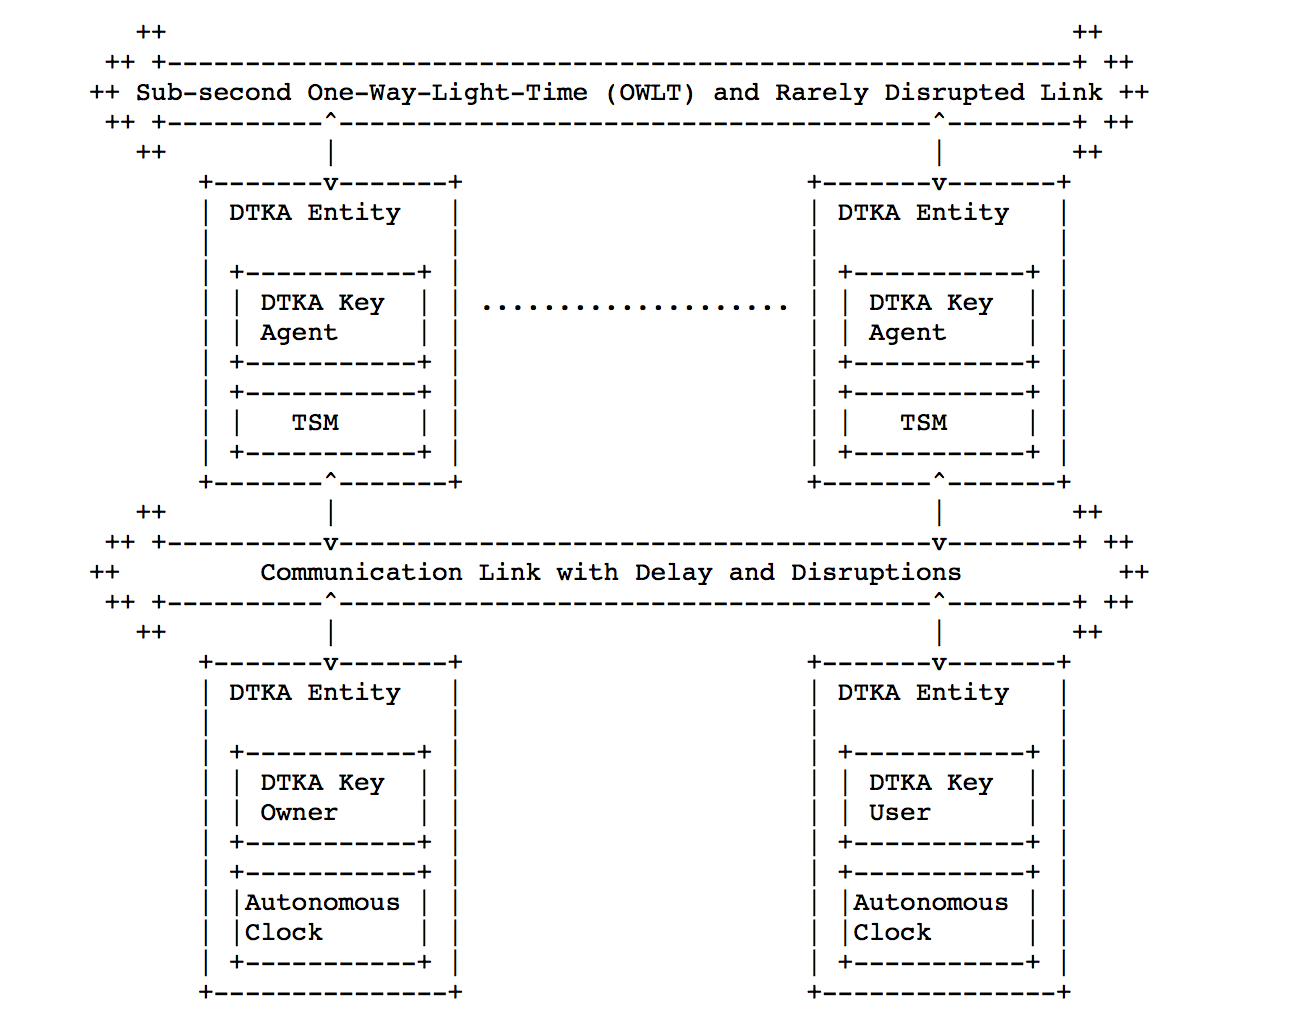
\includegraphics[width=1 \linewidth, height=9.5cm]{images/DTKA.png} 
\caption{DTKA System interactions, \cite{burleigh-dtnwg-dtka-01}}
\label{fig:dtka}
\end{figure}

Each KO generates its private-public pair and has a unique endpoint ID. There are two options to authenticate public keys. In the first option, KO sends an association message via an OOB physical channel signed with the KO private key. In the second option, the KO or a trusted third-party sign a new in-band association request with the private key corresponding to the previous authenticated public key. The first time a node register with the Key Authority the OOB approach is required. The signature of the KO is not for authentication, and it is only to prove that the node is in possession of the private key corresponding to the public key. Authentication requires a manual check of the message received via the physical channel.   




\begin{figure}[htb]
\centering
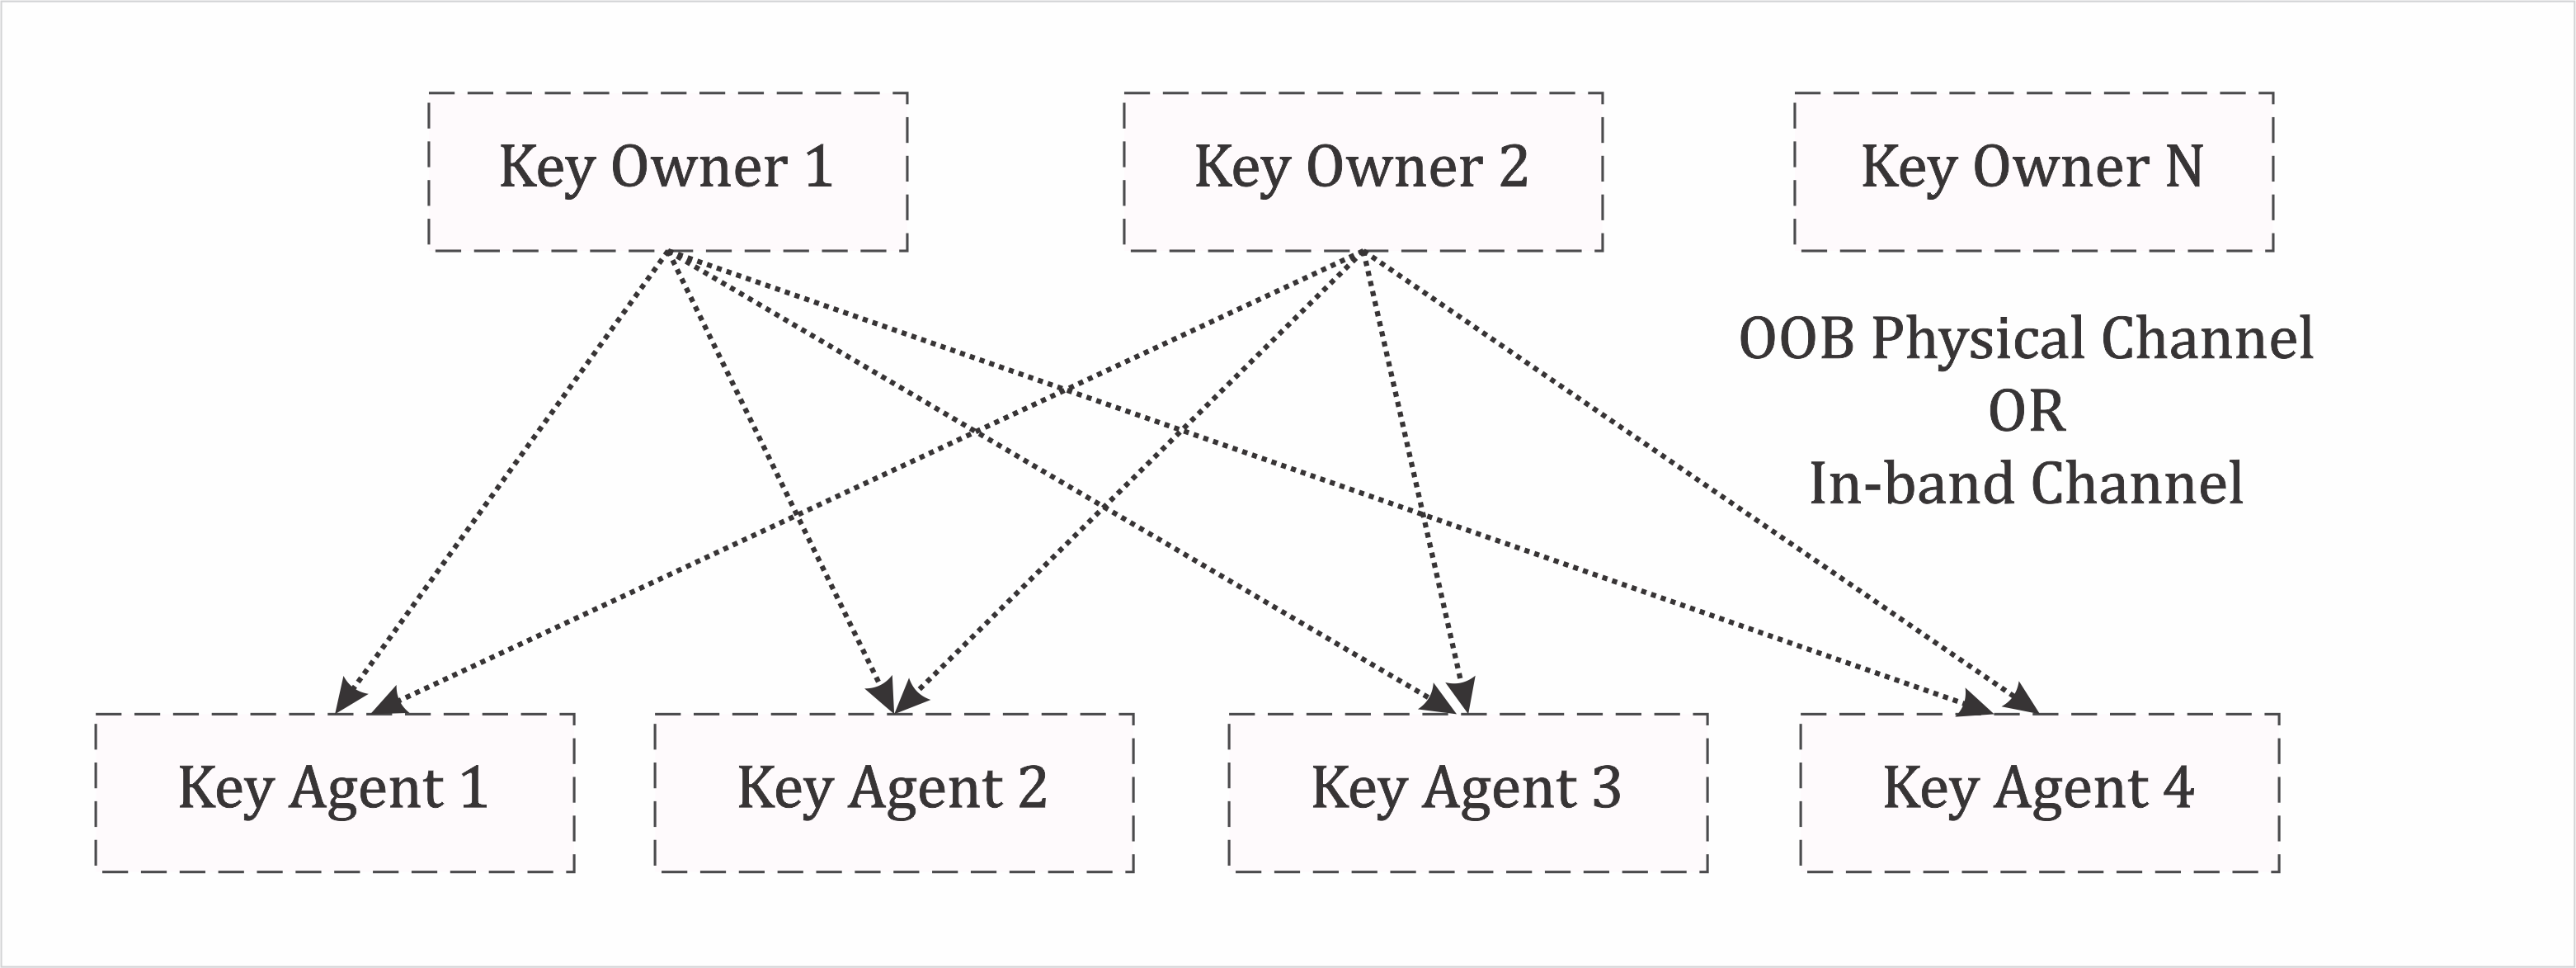
\includegraphics[width=1 \linewidth, height=9.5cm]{images/node-regist.png} 
\caption{Node registration}
\label{fig:Node registration}
\end{figure}


Nodes can periodically renew their public-private key pairs following the ``key roll-over protocol''. The roll-over protocol is similar to the registration process but does not require the OOB channel and the current private key is used to sign the association request.  This request has to be sent to all KAs present in the application domain.

The revocation procedure requires a human operator to initiate the process. The operator authenticates to the respective KA, identify the public key, and instruct a schedule revocation message. The KA then send out the message to all other KA instructing to include the revocation message in the next bulletin.   


Key Agents collect multiple association and revocation request from different parties. Then the KAs reach consensus on the bulletin content. This consensus is the reason why the delay between Key Agents must be under sub-second OWLT. Each DTKA multicast part of the bulletin (code blocks) to all KUs. When a KU receives a code block, it has to verify the authenticity of the message before accepting it. After accepting some code blocks (t-out-n threshold), the KUs can decode the content of the bulletin and store the information locally. 


An association block contains a single pair node ID-public key or a revocation pair. A bulletin is a collection of association blocks. Each bulletin contains a serial number, which is a unique and sequential identifier, and a trust model value representing the configuration to validate a bulletin. For instance, a list of KAs designated for the bulletin and t-out-n threshold configuration. Finally, a hash is computed over all association blocks of the bulletin. Once the bulletin is complete, a (Q+R)-erasure code algorithm is used to encode the bulletin. 

Each KA is responsible for the distribution of a subset of code blocks and has the backup responsibility for others. DTKA entities receive the configuration of code-block assignments for each KA at system initialisation. Other defence mechanisms are introduced to deal with compromised KAs. The reader is refer to \cite{burleigh-dtnwg-dtka-01} for further details.

In summary, the multicast distribution supports message authentication to avoid spurious bulletins and redundancy to ensure that a minimal set of KAs multicast the information. These, along with other mechanism mention before, minimises the likelihood of clients being unable to decode the bulletin and store the information locally. Each code block is the payload of a bundle protected with a Block Integrity Block from BSP. For that reason, the bulletin does not contain any signature. 

If a node detects gaps in the received code blocks, it must send a message to all KAs requesting the retransmission of the missing code blocks corresponding to a serial number. Upon receiving enough number of code blocks, the KU can reconstruct the bulletin with its unique serial number. After receiving the bulletins, DTN nodes have authenticated public information that can be used to encrypt and authenticate messages during the effective time for each pair node ID-public key. 

A potential problem occurs when an application domain has more than one operating KA. In this case, a KO has to send the association requests to all KAs via an OOB physical channel. Many Key agents provide fault tolerance, so it is safe to assume that KAs will be in different locations. This strong authentication mechanism is proper for sensitive space node such as relay satellites, but it seems an overwhelming overhead for lightwave nodes like a sensor or robot. Even more, DTN nodes could be anything from a spacecraft to a process running is an Operating System. A hierarchical approach could work better in this situation where some nodes are required to authenticate with all KAs in their application domain, but less critical nodes could authenticate with one KA. 

\subsection{Other perspective of Key Management}

Recently, Menesidou and Vasilios \cite{menesidou2016automated} study the problem of key management on opportunistic networks. They argue that key management is better exploited when used in conjunction with routing decision by DTN security aware nodes. They used the critical path method CPM as a decision making method for path different path between source and destination in which the duration of each activity is the end-to-end delay. The critical path represent the path with longest delay. The idea is that security aware nodes can exploit the slack time to perform key management operations. The authors developed a protocol parser for evaluating complex scenarios and simulate a space DTNs.

Most of the proposal study in this section are based on traditional public certificates, Identity-based Cryptography. Rusch \textit{et al.}  \cite{rusch2017forward} propose using puncturable encryption constructions for highly asynchronous scenarios. Their scheme ensures forward secrecy of messages at the cost of higher latency. Recipients nodes repeatedly update the decryption keys to revoke decryption capabilities for selected time intervals, recipients or messages. The authors assumed that exist an infrastructure for key exchange, but their system uses FSE public keys instead of RSA public keys. There is no mention of initialisation or distribution in this work.


Group key management is an option for multicast communication. This project does not focus on group communication, but a brief analysis of some works is presented. Groups key management can be classified into centralised, decentralised and distributed. The critical security requirement for group key management are forward secrecy, backward secrecy, collusion freedom and key independence \cite{camtepe2005key}. 


Xu \textbf{et al.} \cite{xu2012chinese} propose a group key management mechanism based on the Chinese Remainder Theorem for DTNs. The advantages are that the system does not need to broadcast messages when a node joins the domain, and only send one message when a node leaves the domain. A stateless scheme is used in this work to overcome delays and high error rates. For many to many communication, they add a lifetime to the group key to deal with users leaving the group. If a node does not receive the key update message at the corresponding interval, it can direct inquiry to a neighbour reducing the latency, but this is unacceptable for space-based networks REQ 2.

Another approach is proposed by Zhou \textbf{et al.} \cite{zhou2014autonomic} based on one-encryption multi-decryption key protocol for deep space. Authors claim that their scheme is more efficient than previous ones, but the join and leave operation could be done without the authority in violation of REQ 2. They argue that the operation has the property of forward-security and backward-security if the key independence condition holds.
